\subsection{ Marco Conceptual}
\subsubsection{\textbf{Android}}
Sistema operativo basado en Linux, fue desarrollado para dispositivos móviles con pantalla táctil, al día de hoy es el sistema operativo más usado del mundo por encima de Ios de Apple. Los dispositivos con este sistema operativo se puede programar en Java o en Kotlin.\\

\subsubsection{\textbf{NoSql}}
Son muchas las aplicaciones web que utilizan algún tipo de bases de datos para funcionar. Hasta ahora estábamos acostumbrados a utilizar bases de datos SQL como son MySQL, Oracle o MS SQL, pero desde hace ya algún tiempo han aparecido otras que reciben el nombre de NoSQL (Not only SQL – No sólo SQL) y que han llegado con la intención de hacer frente a las bases relacionales utilizadas por la mayoría de los usuarios \citeW{acens_2018}.\\
Ventajas:\\
Esta forma de almacenar la información ofrece ciertas ventajas sobre los modelos relacionales. Entre las ventajas más significativas podemos destacar:
\begin{itemize}
\item Se ejecutan en máquinas con pocos recursos: Estos sistemas, a diferencia de los sistemas basados en SQL, no requieren de apenas computación, por lo que se pueden montar en máquinas de un coste más reducido.
\item Escalabilidad horizontal: Para mejorar el rendimiento de estos sistemas simplemente se consigue añadiendo más nodos, con la única operación de indicar al sistema cuáles son los nodos que están disponibles.
\item Pueden manejar gran cantidad de datos: Esto es debido a que utiliza una estructura distribuida, en muchos casos mediante tablas Hash.
\item No genera cuellos de botella: El principal problema de los sistemas SQL es que necesitan transcribir cada sentencia para poder ser ejecutada, y cada sentencia compleja requiere además de un nivel de ejecución aún más complejo, lo que constituye un punto de entrada en común, que ante muchas peticiones puede ralentizar el sistema.
\end{itemize}

\subsubsection{\textbf{Arquitectura Limpia}}
Robert Martin, más conocido como Tío Bob (Uncle Bob en inglés), plantea que la arquitectura de un software debe gritar cuál es el uso de dicho software. Así como al ver planos de edificios, si uno ve que el edificio posee un baño, cocina, comedor, dormitorios, la arquitectura grita que es una casa familiar. De esta manera, al visualizar la arquitectura de un software, se debería notar cual es el uso del mismo. La arquitectura no debería indicar cuál es el framework o herramientas usadas para su construcción.

Volviendo al arquitecto de edificios, el mismo se asegura que un edificio cumpla con los casos de uso antes de decidir qué materiales se usarían para su construcción. En el caso del desarrollo de software, cumplimentar esto, asegura que el producto satisfaga los casos de uso y retrase la decisión sobre los frameworks o herramientas a usar. Incluso, una buena arquitectura basada en casos de usos permite que sea fácil cambiar la herramienta que se va a usar \citeW{clean-architecture_2018}.

\begin{figure}[h]
\centering%
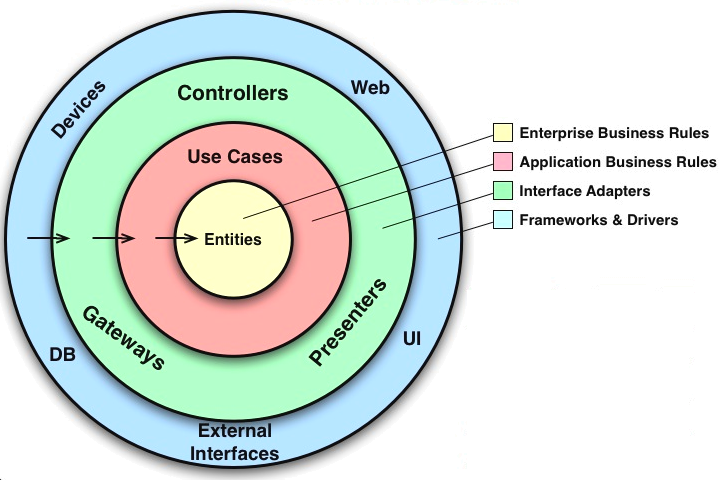
\includegraphics[width=\textwidth,keepaspectratio=true]{contextualizacion/MarcoReferencial/imgs/clean_architecture.png}%
\caption{Arquitectura Limpia.} \label{fig:clean_architecture}
\end{figure}


La propuesta del Tío Bob sobre la arquitectura limpia impone las siguientes restricciones:\\

\begin{itemize}
\item \textbf{Independiente de frameworks:} la arquitectura no debe atarse a las restricciones del framework. Esto permite considerar al framework como una herramienta.
\item \textbf{Testeable:} las reglas de negocios deberían poder probarse independientemente de la UI, base de datos u otras herramientas.
\item \textbf{Independiente de la UI:} la interfaz de usuario se debería poder cambiar fácilmente sin necesidad de cambiar la lógica de negocio.
\item \textbf{Independiente de la base de datos:} las reglas de negocios no deberían estar ligadas a la base de datos o herramienta de persistencia.
\end{itemize}

\subsubsection{\textbf{MVP}}
Es una derivación del patrón arquitectónico modelo–vista–controlador (MVC), y es utilizado mayoritariamente para construir interfaces de usuario\\
En MVP el presentador asume la funcionalidad del "intermediario". En MVP, toda lógica de presentación es colocada al presentador \citeW{mvp_2018}.\\
MVP es un patrón arquitectónico de interfaz de usuario diseñada para facilitar pruebas de unidad automatizada y mejorar la separación de inquietudes en lógica de presentación:
\begin{itemize}
\item El modelo es una interfaz que define los datos que se mostrarán o no actuado en la interfaz de usuario.
\item El presentador actúa sobre el modelo y la vista. Recupera datos de los repositorios (el modelo), y los formatea para mostrarlos en la vista.
\item La vista es una interfaz pasiva que exhibe datos (el modelo) y órdenes de usuario de las rutas (eventos) al presentador para actuar sobre los datos.
\end{itemize}

\subsubsection{\textbf{SISTEMAS DE RECOMENDACIÓN}}
Es un sistema inteligente que proporciona a los usuario sugerencias personalizadas sobre un determinado tema. Estudian el perfil del cliente, sus búsquedas anteriores, sus compras, perfiles, páginas visitadas, recopilan toda esta información e intentan hace sugerencias que son de interés del usuario.\\

Uno de los sistemas de recomendación famosos son, Amazon e Youtube, la primera utiliza la información de las compras de los usuarios, la navegación y búsqueda de los productos para sugerir posibles productos de interés. Youtube registra la búsqueda de vídeos y la visualización de vídeos para mostrar sugerencias de vídeos que le podrían gustar.
\citeW{Quesonl99:online}

Los sistemas de clasificación se pueden dividir en 4 tipos:  

\begin{enumerate}
\item \textbf{Filtrado basado en Contenido} Las recomendaciones se basan en el conocimiento que se tiene sobre los items que el usuario ha valorado (ya sea de forma implícita o explícita), y se le recomendarán items similares que le puedan gustar o interesar. Un ejemplo de es Youtube.
\item  \textbf{Filtrado Demográfico:} Estas recomendaciones se realizan en función de las características de los usuarios (edad, sexo, situación geográfica, profesión, etc).
\item \textbf{Filtrado Colaborativo:} Consiste en ver que usuarios son similares al usuario activo (o usuario al que hay que realizarle las recomendaciones) y a continuación,recomendar aquellos items que no han sido votados por el usuario activo y que han resultado bien valorados por los usuarios similares. Un ejemplo de es Filmaffinity.
\item \textbf{Filtrado Híbrido}:  Mezclan alguno de los tres filtrados mencionados anteriormente para realizar recomendaciones e incluso lo combinan con alguna otra técnica de inteligencia artificial como pueda ser la lógica borrosa o la computación evolutiva. Un ejemplo es Amazon.
\end{enumerate}


\begin{figure}[htbp]
\centering%
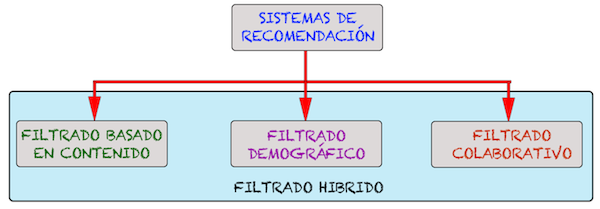
\includegraphics[width=\textwidth,keepaspectratio=true]{contextualizacion/MarcoReferencial/imgs/Sistema-de-Recomendacion-Clasificacion-jarroba.png}%
\caption{Tipos de sistema de recomendación.\citeW{Quesonl99:online}} 

\label{fig:sisrec}
\end{figure}

\subsubsection{\textbf{MICROSERVICIOS}}
Se define un microservicio es una pequeña aplicación que puede ser desplegada, probada y escalada de forma independiente y que tiene una única responsabilidad\cite{7030212}. Hablamos de única responsabilidad en su definición básica, que es que solo se tenga que cambiar por sola una cosa \cite{Martin:2008:CCH:1388398}.

\subsubsubsection{\textbf{\textit{¿Qué se debe tener en cuenta?}}}

Se espera que un microservicios no tengo muchas líneas de código y puedas entrar todo su poder a sólo una funcionalidad. Normalmente cuando se empieza en un proyecto, se inicia con una aplicación monolítica, que para un inicio están bien, pero a medida que el proyecto va creciendo se vuelve más complicado su mantenibilidad, su escalabilidad, sus pruebas debido a que todos los proyectos los servicios están unidos, haciendo que los despliegues se vuelvan complicados y muy grandes. Al tener una aplicación monolítica, hace que un fallo en uno de los servicios puede tumbar toda nuestra aplicación, una cosa que no deseamos. Y también si queremos hacer un pequeño cambio en nuestro código significa que tenemos que desplegar toda la aplicación, no se puede desplegar sobre el pequeño cambio que hicimos. Estos son unos de los problemas que intenta atacar la arquitectura por microservicios, y por lo cuál en los últimos tiempos se han vuelto tan utilizada, haciendo servicios compactos e independientes hacemos que se pueda tomar ventaja de todas las tecnologías que hay en el mercado pudiendo a cada uno de los servicios especializarlo en la tecnología que más le convenga, estos servicios son especializados, o sea que sólo tienen una una responsabilidad lo cual los hace fácil de escalar de mantener y de probar. Un módulo común de esta arquitectura es que tenga la lógica de negocio asociado con la base de datos la base de datos Y es única para ese servicio, esto implica que si queremos hacer un cambio en ese servicio sólo tenemos que desplegar ese servicio sin afectar los demás, asimismo, si un servicio falla todos los otros servicios de nuestra aplicación pueden seguir funcionando \citeW{Microser90:online}.

\subsubsubsection{\textbf{\textit{¿Es buena idea iniciar de una con microservicios?}}}

Cuando se decide implementar una arquitectura por microservicios debe tener muy claro la lógica del negocio, porque hay que saber muy bien cómo se va a dividir el proyecto en los diferentes servicios, en cada uno de los servicios para así no tener problemas más adelante, la mayoría de empresas que han implementado microservicios, lo primero que han tenido es una aplicación monolítica, una aplicación con todos sus servicios integrados y a medida que van creciendo y ya con la lógica de negocio clara, definen los servicios que necesitan y empiezan a dividir su código monolítico en servicios más pequeños y especializados \cite{Dragoni2017}. 

\subsubsubsection{\textbf{\textit{¿Es compleja la migración?}}}

La respuesta concisa es que si, al tener muchos microservicios empezamos a tener necesidades que no teníamos antes con las aplicaciones monolíticas, tenemos que tener en cuenta que pueden ser muchos servicios que se van a estar comunicando entre ellos y hacia el exterior, aquí es donde nos empieza a apoyar todas las herramientas de despliegue continuo y computación en la nube, al tener muchos servicios nos encontramos con el inconveniente de tener que hacer muchos despliegues y muchas configuraciones en ambientes separados lo cual sin herramientas que nos ayuden a esta tarea sería muy complicado de mantener, adicionalmente pensando en la escalabilidad de un sistema nos damos cuenta de que esos servicios se pueden duplicar, triplicar, ...,  dependiendo de la carga dependiendo lo que de las configuraciones que tengamos, lo cual hace que no podemos tener direcciones o apuntador servicios estáticos, tenemos que tener herramientas o servicios que nos permitan dinámicamente encontrar todos los microservicios de nuestra aplicación, con esto queremos decir que una aplicación de microservicios no es sólo dividir servicios y ya, detrás de eso tenemos lógicas esenciales y herramientas para que esto pueda funcionar la forma correcta y que no se nos vuelva un problema al final. Para esto vamos a utilizar toda la parte de integración continua y adicionalmente servicios de Gateway que nos permitan encontrar y distribuir nuestros servicios \citeW{Microser11:online}\cite{Dragoni2017}.
